\section{Visualisation des resulats expérimentaux - modèle physique}
\subsection{Visualisations}
\begin{frame}
    \frametitle{Quelques visualisations 1/3}
    \begin{figure}[!h]
        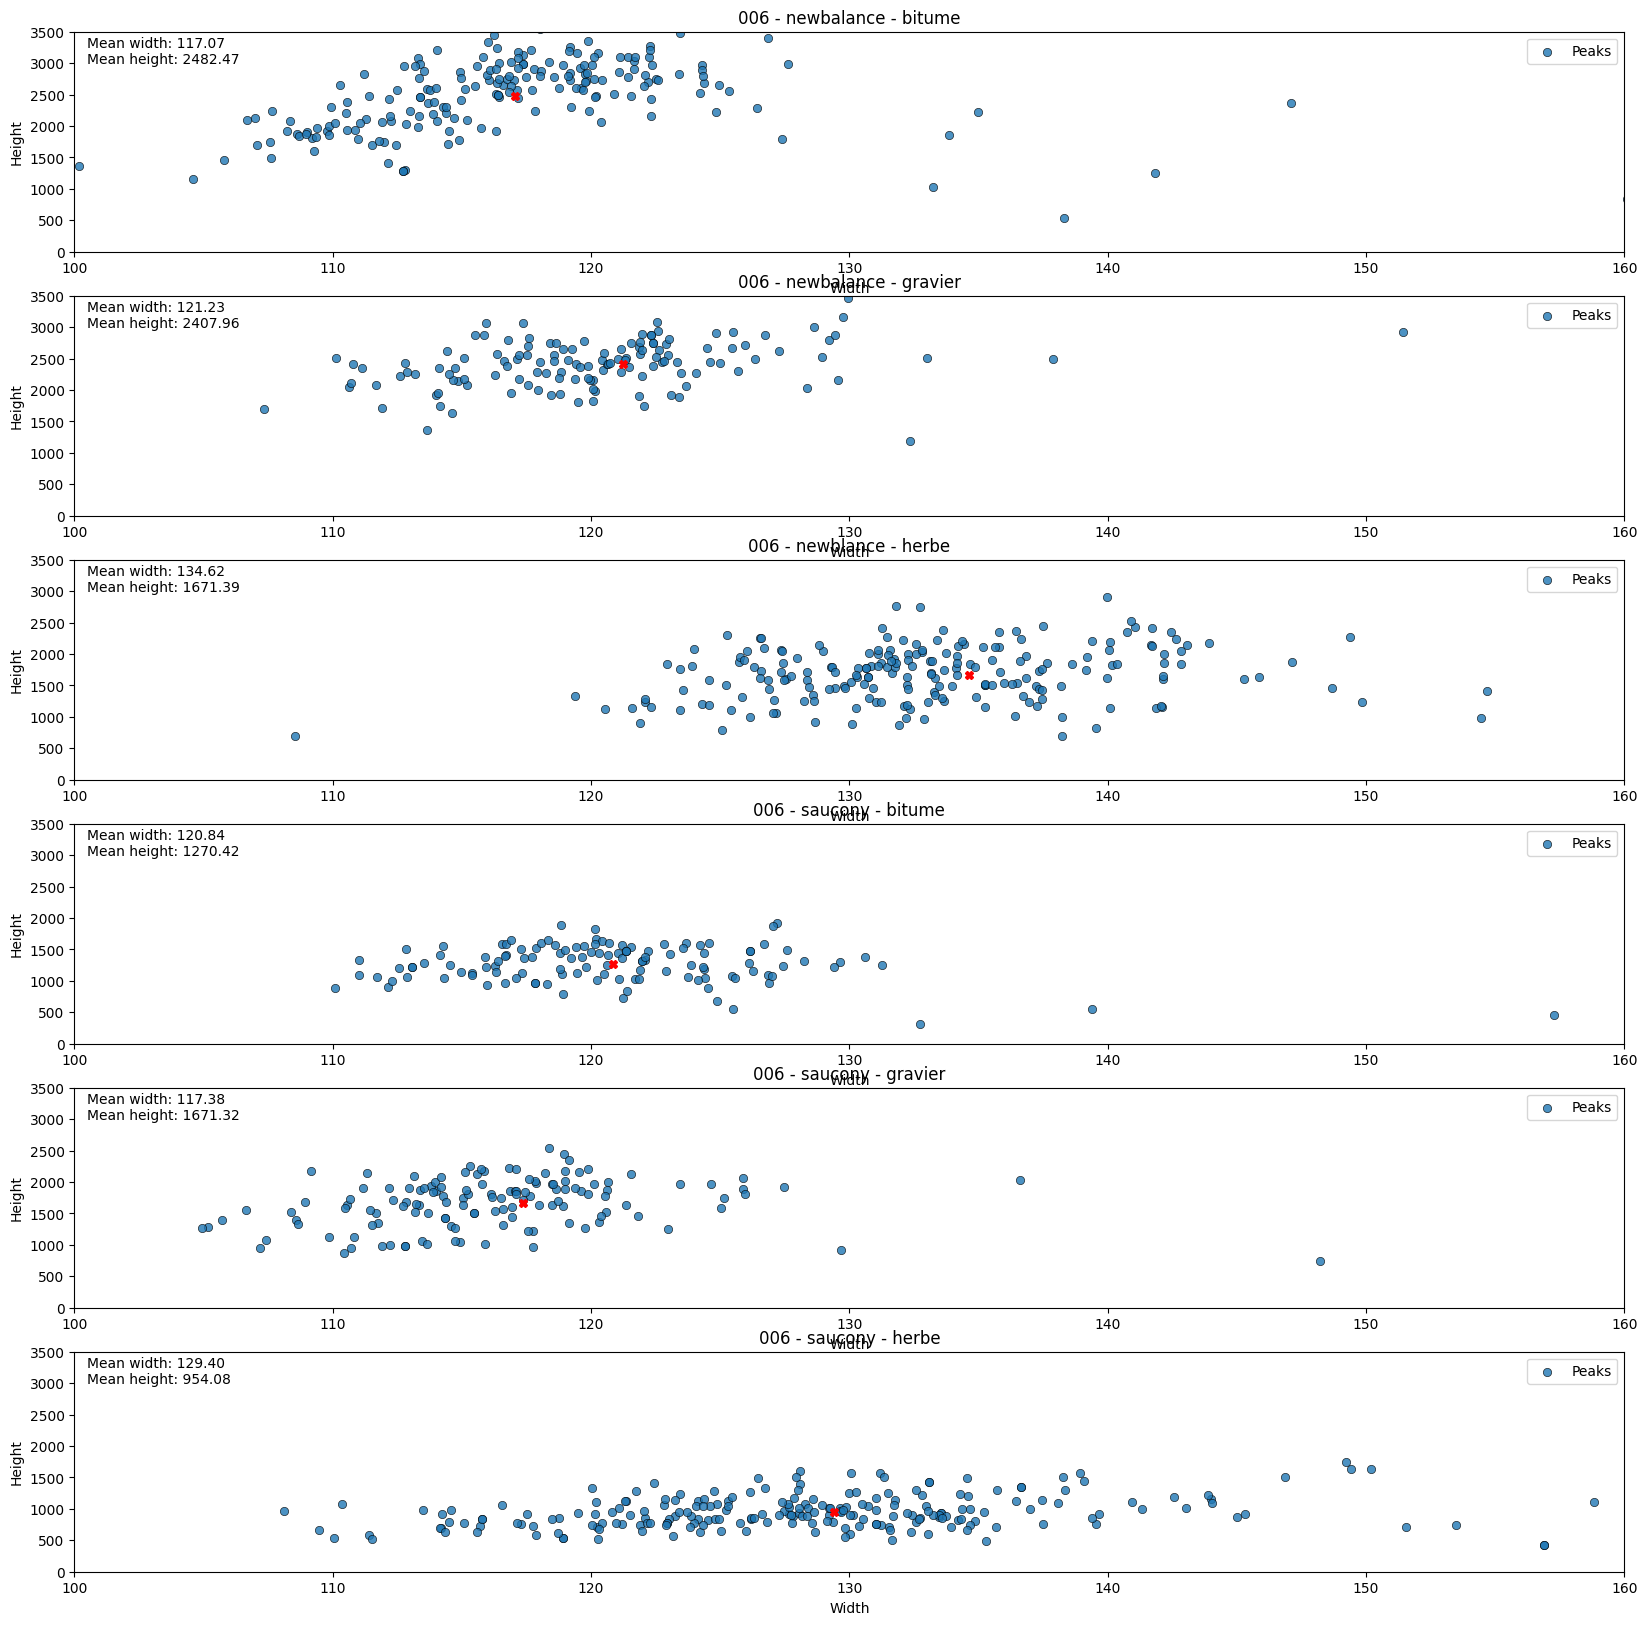
\includegraphics[scale=0.2]{./figures/res_02.png}
    \end{figure}
\end{frame}
\begin{frame}{Quelques visualisations 2/3}
    \begin{figure}
        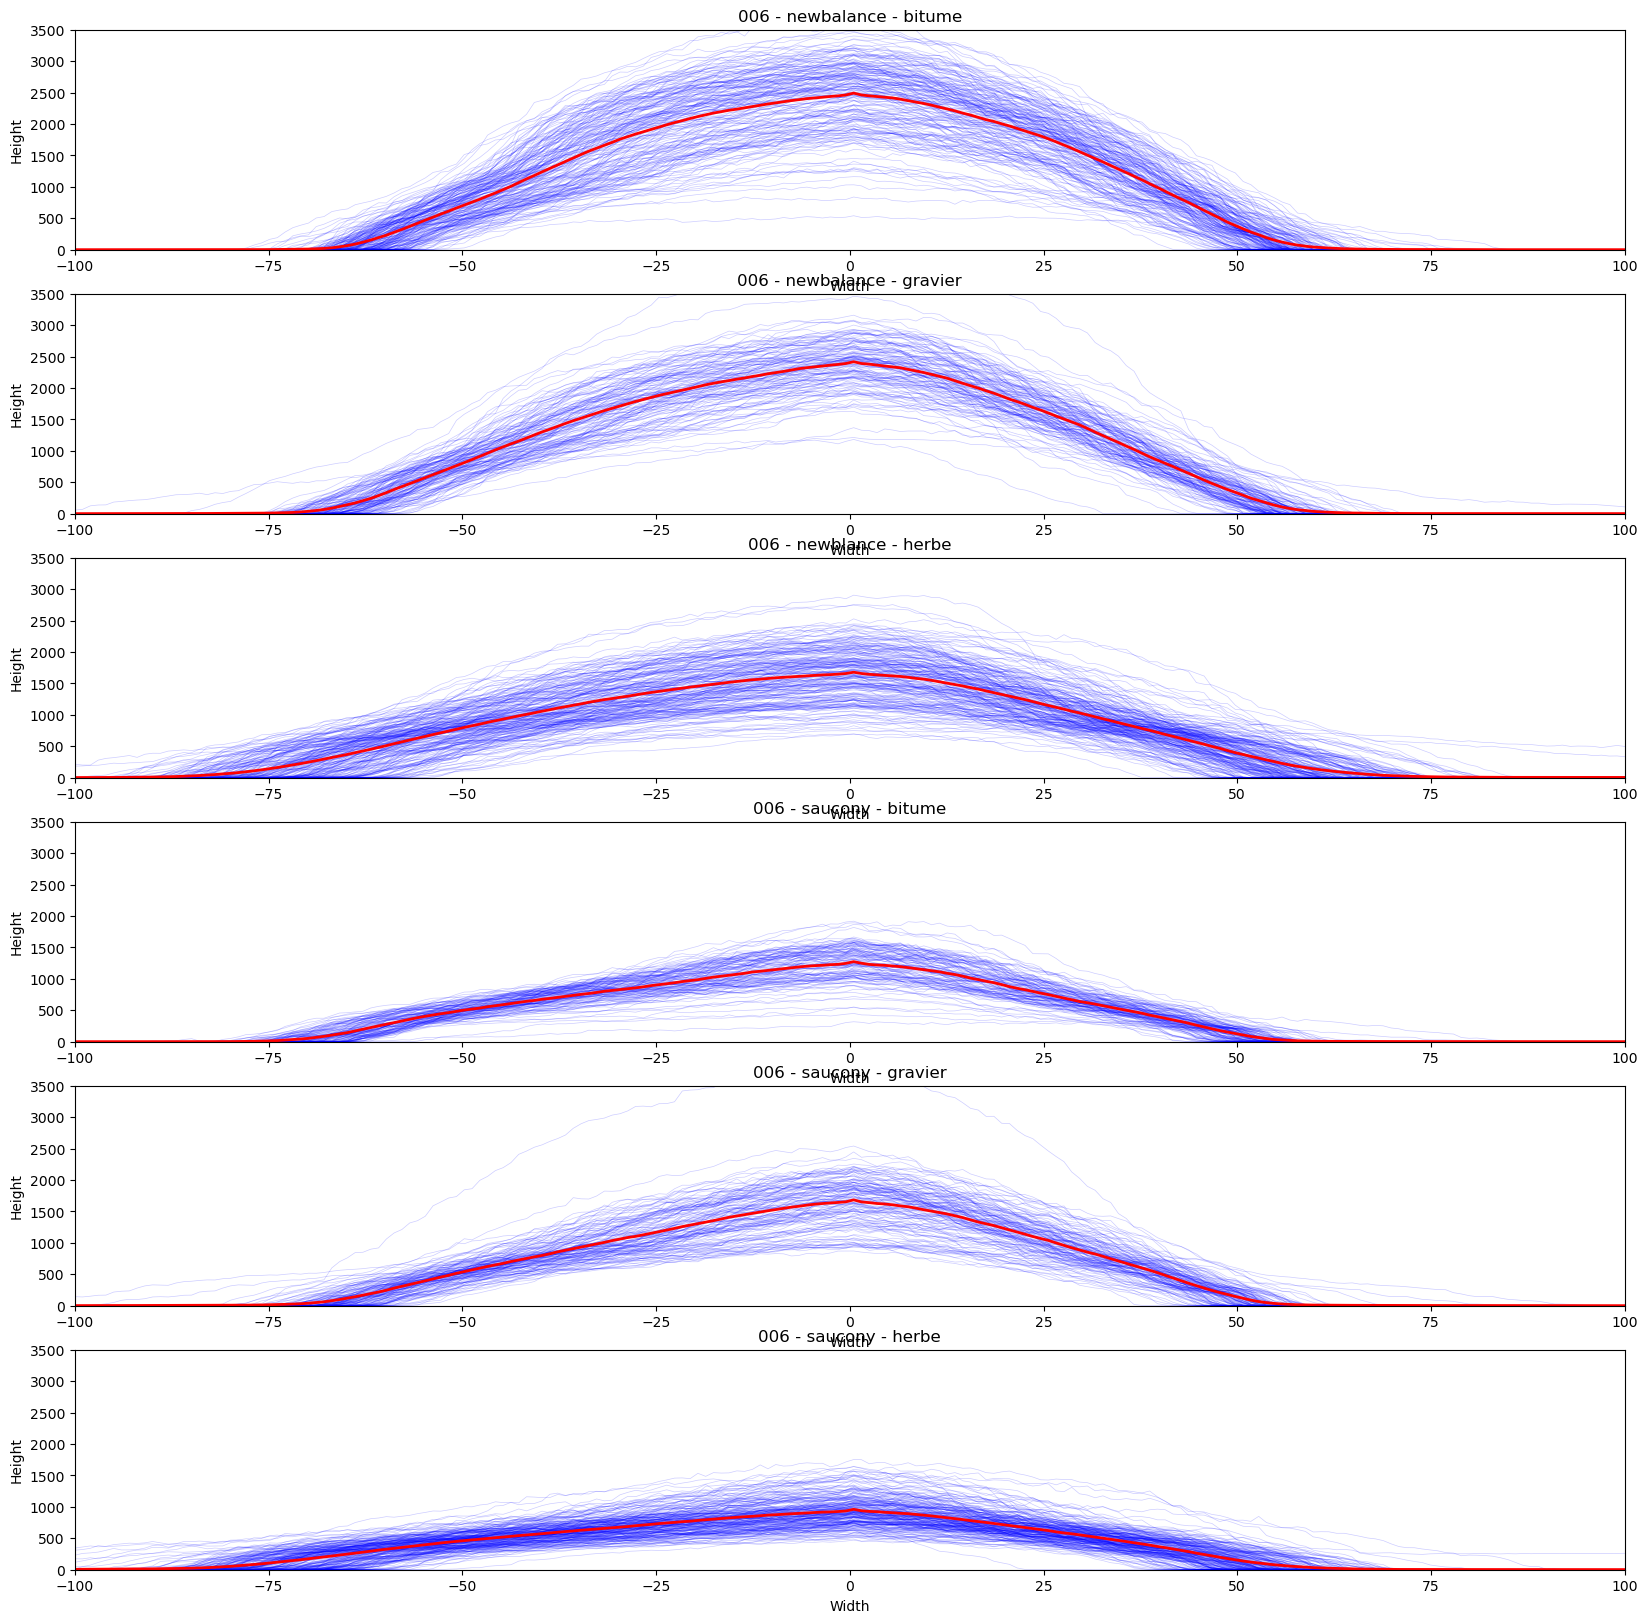
\includegraphics[scale=0.2]{./figures/res_03.png}
    \end{figure}
\end{frame}
\begin{frame}{Quelques visualisations 3/3}
    On garde maintenant les courbes moyennes pour chaque revètement:
    \begin{figure}
        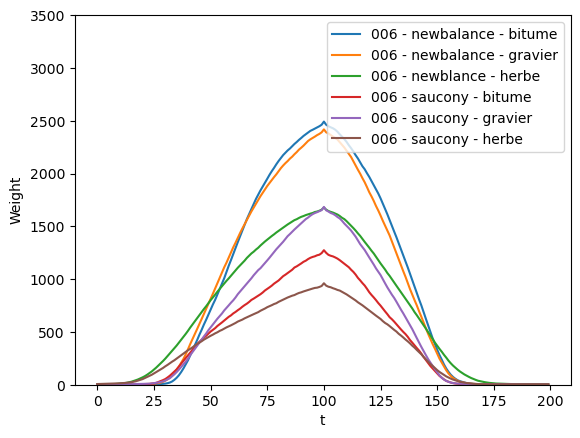
\includegraphics[scale=0.5]{./figures/res_04.png}
    \end{figure}
\end{frame}
\subsection{Modèle physique}
\begin{frame}{Rhéologie}
    L'os est un matériaux viscoélastique, on adopte le modèle de Kelvin-Voigt:
    \begin{figure}
        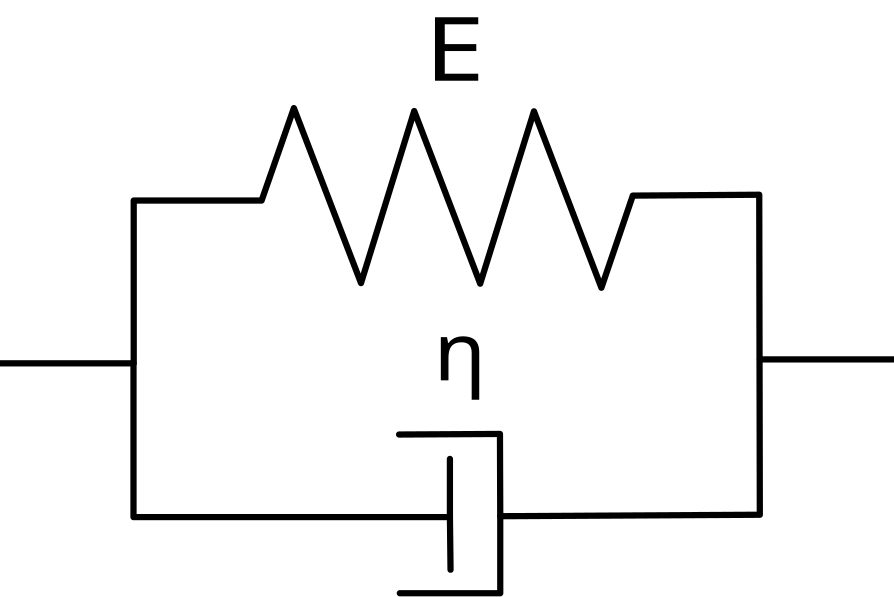
\includegraphics[scale=0.1]{./figures/rheo_00.png}
    \end{figure}
    On établit l'équation différentielle suivante:
    $$ \sigma = E \times \varepsilon + \eta \times \frac{d\varepsilon}{dt}$$
    Et la fonction de transfert associée:
    $$ H(\omega) = \frac{1}{E+i\omega\eta}$$
\end{frame}
\begin{frame}{Résultats}
    Après avoir appliqué la transformée de Fourier aux données et utilisé la fonction de transfert, on obtient:
    \begin{figure}
        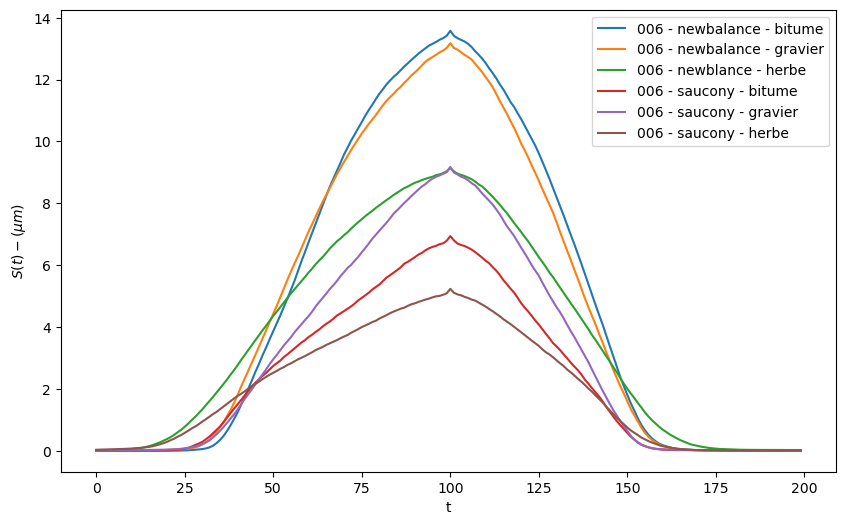
\includegraphics[scale=0.5]{./figures/rheo_05.png}
    \end{figure}
\end{frame}
